\documentclass[12pt, letterpaper]{article}
\usepackage[margin=1in]{geometry}
\usepackage{amsmath, amssymb, amsthm}
\usepackage{enumitem}
\usepackage{hyperref}
\usepackage{listings}
\usepackage{pythonhighlight}
\usepackage{graphicx}
\usepackage[skip=5pt, indent=20pt]{parskip}

\title{CS 2051: Patterns in Primes}
\author{Anthony Hong \\ Georgia Institute of Technology
\and Yongyu Qiang \\ Georgia Institute of Technology
\and Aravinth Venkatesh Natarajan \\ Georgia Institute of Technology}
\date{March 12th, 2023}

%%%%%%%%%%%%%%%%%%%%%%%%%%%%%%%%%%%%%%%%%%%%%%%%%%%%%%%%%%%%%%%%

\begin{document}

\maketitle

\section{Background}
% This section should develop the basic definitions and
% preliminary results required for the statement and proof of
% your main result, including examples that help the reader to
% develop intuition for the concepts presented. Start from scratch, remember your audience is other 2051 students.
(hook to be added here)

A common result many students learn early on in number theory is about the
infinitude of prime numbers. This fact is also known as Euclid's theorem,
and we include a short summary of Euclid's original proof.

\noindent
\textbf{Euclid's Theorem.} \textit{The set of all prime numbers is larger
in cardinality than any finite collection of prime numbers.}

\noindent
\textit{Proof.} Consider $p_1, p_2, \dots, p_n$, some arbitrary finite
collection of
prime numbers. Let $N = p_1p_2 \dots p_n$, and consider $P = N + 1$. $P$ is
either prime or not prime.
\newline\indent
First, let $P$ be prime. Then, we have constructed a new prime number and
we are done.
\newline\indent
Now, let $P$ not be prime. Let $g$ be a prime factor of $P$. We propose that
$g \notin \{p_1, p_2, \dots, p_n\}$. To show this, suppose that
$g \in \{p_1, p_2, \dots, p_n\}$. Then, since $p_1, p_2, \dots, p_n$ are all
factors of $N$, we have $g | N$. $g | P$ and $g | N$, so
we must also have $g | (P - N)$, i.e.\ $g | 1$. But $g > 1$ ($g$ is prime),
so $g$ cannot possibly divide 1. Therefore,
$g \notin \{p_1, p_2, \dots, p_n\}$, and we have found a new prime, as
required. \hfill$\square$

A natural next step from here is to explore how prime numbers
are distributed. An important result from the 1890s was the
prime number theorem.

\noindent
\textbf{Definition.} $\pi(n)$ (move definition of $\pi(n)$ here)

\noindent
\textbf{Prime Number Theorem.} (move statement of PMT here)

However, due to its reliance on tools from analysis, we'll
forgo a proof of the prime number theorem in this paper.

(Begin discussion of prime gaps)

(Start with small prime gaps) \\
(Give proof that finitely many odd prime gaps exist since one of
$n$ and $n + k$ must be even for odd $k$) \\
(Introduce Twin Prime Conjecture)

(Discuss large prime gaps) \\
(Give proof for arbitrarily large prime gaps using $n! + 2,
n! + 3, \dots, n! + n$) \\
(Talk about how the previous result is actually not nearly the
best we can do, maybe give a pigeonhole principle argument
about a better bound that grows faster)

\section{Cram\'er's Random Model}
% In this section, you should state and prove your main result,
% and provide some basic consequences and examples that help the
% reader to understand it. You may want to change this section's
% name to something more informative.
A interesting problem is the rate of growth of prime gaps. $\pi(n)$ denotes the prime counting function, which counts the number of primes less than or equal to $n$. The Prime Number Theorem (PMT) states that $x / \ln(x)$ approximates $\pi(n)$. To be more precise, the PMT states: \[\lim_{x \to \infty} \frac{\pi(x)}{\left\lfloor \frac{x}{\ln(x)} \right\rfloor} = 1\]
This means, as x gets larger, $x / \ln(x)$ will get better as an approximation for $\pi(x)$. This also implies that the average size of the gaps between consecutive primes up until $x$ asymptotically approaches $\ln(x)$. So for a random number $n$ in the interval $[x, x + kx]$ for large $x$ and fixed $k$, the probability that $n$ is prime is approximately $1 / x \approx 1 / n$.

Cram\'er's random model uses this idea as a naive approach to emulate the distribution of prime numbers. Consider a random subset of the natural numbers, where the independent probability that a number $n$ is chosen is $1 / \ln(n)$. Let's call this random set $P'$, where $P$ is the set of actual prime numbers. Cram\'er conjectured that $P'$, which consists of our ``fake primes", accurately models the distribution of P. 

% Perhaps add summary of proof for this result
According to this heuristic, we have the resulting claim, which is known as Cram\'er's conjecture:
\[\limsup_{n \to \infty} \frac{p_{n + 1} - p_n}{(\ln p_n)^2} = 1\]
where $p_n$ denotes the $n$-th prime.

(Some directions to take these ideas):
\begin{itemize}
  \item Problems with Cram\'er's naive model and ways we can improve it (with modern results)
  \item How Cram\'er's model fares depending on the size and location of the interval, calculating asymptomatic statistics
\end{itemize}

\section{Bertrand's Postulate}
Another problem in number theory is finding the bounds in which you would find a prime number. Of these, one of the paramount significance is \textbf{Bertrand's Postulate}: \\
Bertrand's postulate states that for an integer $i > 1$, there is at least one prime number $p$
\[
    i \leq n \leq 2i 
\]
The proof for it is as follows:\\
We'll start by proving Lemma 1:\\
\[
    \frac{4^n}{2n} \leq {2n \choose n}
\]
\[
    4^n = (1 + 1)^{2n} = \sum{k = 0}^{2n} {2n \choose k} 
\]
Since, $2n \choose 0$ is 1 and $2n \choose 2n$ is 1, this is the same as
\[
    \equiv 2 + \sum{k = 1}^{2n - 1} {2n \choose k} 
\]
Since the largest term in this summation is $2n \choose n$ (since for $n \choose k$, $k = n/2$ will give the largest term) and there are $2n$ terms, 
\[
     (2 + \sum{k = 1}^{2n - 1} {2n \choose k}) \leq (2n * {2n \choose n})
\]
Therefore, 
\[
    \frac{4^n}{2n} \leq {2n \choose n}
\]
Let's now prove Lemma 2:\\
For a given prime $p$, let's define $r$ as the greatest number for which $p^r | {2n \choose n}$. Lemma 2 is as follows, for such an r, 
\[
    p^r \le 2n
\]
Firstly, we have to introduce Legendre's Formula:\\
Legendre's Formula states that for any prime number $p$, and any integer $n$, let's define the function $v_p(n)$ as the exponent of the largest power of $p$ that divides $n$. Let L = $\left\lfloor \log_{p}{n} \right\rfloor$\\
Legendre's Formula is:
\[
    v_{p}(n!) = \sum_{i = 1}^{L} {\left\lfloor \frac{n}{p^i} \right\rfloor}
\]
${2n \choose n}$ can also be written as $\frac{(2n)!}{n!*n!})$\\ Finding the largest exponent of $p$, $r$, that divides $\frac{(2n)!}{n!*n!}$ is the same as finding the largest exponent of $p$, $r$, that divides each component of $\frac{(2n)!}{n!*n!}$, i.e. $(2n)!$, $n!$\\

In this case, $L = \left\lfloor \log_{p}{2n} \right\rfloor$\\ Writing this in terms Legendre's Formula, we get that:
\[
    v_{p}({2n \choose n}) = \sum_{i = 1}^{L} {\left\lfloor \frac{2n}{p^i} \right\rfloor} - 2\sum_{i = 1}^{L} {\left\lfloor \frac{n}{p^i} \right\rfloor}
\]
This is equivalent to:
\[
    v_{p}({2n \choose n}) = \sum_{i = 1}^{L} {\left\lfloor \frac{2n}{p^i} \right\rfloor - 2\left\lfloor \frac{n}{p^i} \right\rfloor}
\]
Thinking intuitively, every term in $\sum_{i = 1}^{L} {\left\lfloor \frac{2n}{p^i} \right\rfloor - 2\left\lfloor \frac{n}{p^i} \right\rfloor}$ must either be 0 or 1.\\
If ($\frac{2n}{p^i}$ mod 1) $\geq$ 0.5 then the term would be 1, otherwise the term is 0. Therefore, the maximum value of this function would be if all the terms were equal to 1. Since we are only dealing with positive numbers, and the exponent is a monotonic function if both numbers are positive numbers,
\[
    v_{p}({2n \choose n}) = r \leq L
\]
\[
    \equiv r \le \log_{p}{2n}
\]
Therefore, it follows that
\[
    p^r \le p^{\log_{p}{2n}} = 2n
\]
We are able to prove our initial Lemma 2, 
\[
    p^r \le 2n
\]
(We will proceed to prove Lemma 3 and 4, which will, in combination prove Bertrand's Postulate)

\section{Extending the Model}
% You should change this section's name to something relevant to
% your project (e.g. "Applications of the RSA encryption
% algorithm" or "Linear Diophantine equations in $n$ unknowns"
\begin{itemize}
    \item Connections from Cram\'er's conjecture to the Riemann hypothesis
    \item Other ways to use Cram\'er's technique of random modeling
\end{itemize}


\section{Preliminary Code and Illustrations}
% Here should be some illustration of the concepts described above. Also place any code you used to generate the code (use the lstlisting package if this applies to you).

Cram\'er's random model allows us to heuristically test properties of primes.
In this example, we graphically compare the maximal prime gap of the model and the actual primes.

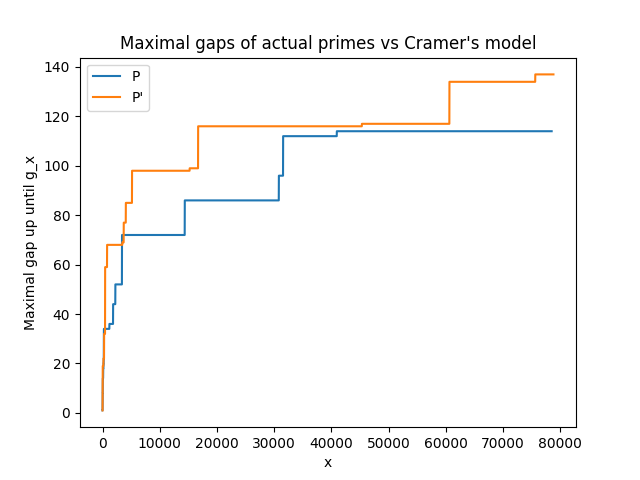
\includegraphics[scale=0.7]{graph.png}
\inputpython{example.py}{6}{40}

\section{Accuracy of the Model}
% You should change this section's name to something relevant to
% your project. This section allows you to reflect or conclude
% the work you have done in your project and discuss future work
% that could be done on the project (e.g. applications you tried
% to make but couldn't find the time).

Under heuristic testing with variations of Cram\'er's model, we should be able to support strong statements such as Bertrand's postulate and Legendre's conjecture. However, comparing with the actual primes, it should be clear that Cram\'er's model is inaccurate. Further work would involve the creation and tuning of other random models, to more closely emulate prime distributions.

\section{References}
% Here you should acknowledge people whose help you are thankful
% for (and why), and any sources such as books and websites that
% you used when studying for the project.

\begin{itemize}
    \item \href{http://terrytao.wordpress.com/2015/01/04/254a-supplement-4-probabilistic-models-and-heuristics-for-the-primes-optional/#more-7956}{Terence Tao's Blog}
    \item \href{https://en.wikipedia.org/wiki/Prime_gap}{Wikipedia}
\end{itemize}

 
\end{document}
